\documentclass[a4paper]{article}
\usepackage[margin=1in]{geometry}%设置边距,符合Word设定
\usepackage{amssymb,amsfonts,amsmath,amsthm}
\usepackage{ctex}
\usepackage{setspace}
\usepackage{lipsum}
\usepackage{graphicx}%插入图片
\usepackage{listings}
\graphicspath{{Figures/}}%文章所用图片在当前目录下的 Figures目录

\usepackage{hyperref} % 对目录生成链接,注:该宏包可能与其他宏包冲突,故放在所有引用的宏包之后
\hypersetup{colorlinks = true,  % 将链接文字带颜色
	bookmarksopen = true, % 展开书签
	bookmarksnumbered = true, % 书签带章节编号
	pdftitle = 例三论文, % 标题
	pdfauthor =刘正浩} % 作者
\bibliographystyle{plain}% 参考文献引用格式
\newcommand{\upcite}[1]{\textsuperscript{\cite{#1}}}

\renewcommand{\contentsname}{\centerline{Contents}} %经过设置word格式后,将目录标题居中

\lstset{
	basicstyle = \small
}

\title{\heiti\zihao{2} 例三论文}
\author{\songti 刘正浩}
\date{\today}


\begin{document}
	\maketitle
	\thispagestyle{empty}

% \begin{abstract}
% 	\lipsum[2]
% \end{abstract}

\tableofcontents
	\section{状态机设计}
		由于采用行为级描述进行例五状态机的设计,设计思路与例二大致相同。\par
		状态机拥有四个输入口与两个输出口,四个输入口分别为两个方向交通灯的控制信号$T_A$与$T_B$,时钟输入$clk$,复位输入$reset$(采用同步复位),
		两个输出口输出位宽为2bit的交通灯状态信号$L_A$与$L_B$。
		\begin{figure}[htbp]
			\centering
			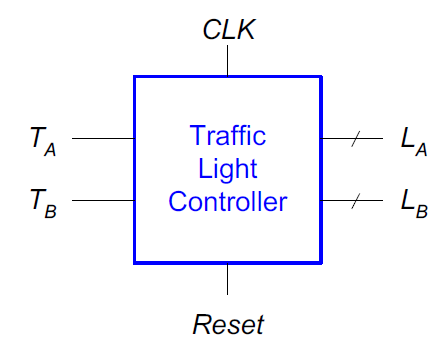
\includegraphics[scale=0.6]{状态机示意图.png}
			\caption{状态机示意图}
		\end{figure}\par
		我们十分熟悉常见的十字路口的红绿灯。在某一时刻,路口的红绿灯可能存在四种状态:
		\begin{itemize}
			\item A方向为红灯,B方向为绿灯
			\item A方向为红灯,B方向为黄灯
			\item A方向为绿灯,B方向为红灯
			\item A方向为黄灯,B方向为红灯
		\end{itemize}
		所以本题中的状态机共有上述四种状态,分别记为$S_A$,$S_B$,$S_C$与$S_D$。再结合控制信号$T_A$与$T_B$,可以得到状态转移图:
		\begin{figure}[htbp]
			\centering
			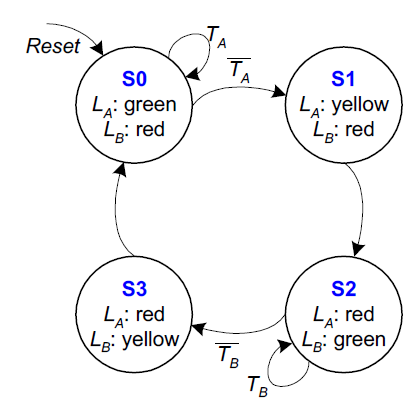
\includegraphics[scale=0.8]{状态转移图.png}
			\caption{状态转移图}
		\end{figure}
		有了状态转移图,就可以用三段式的方法来写出状态机。具体的用$T_A$与$T_B$来控制状态转换的方式请见状态转移表(图3)。
		\begin{figure}[htbp]
			\centering
			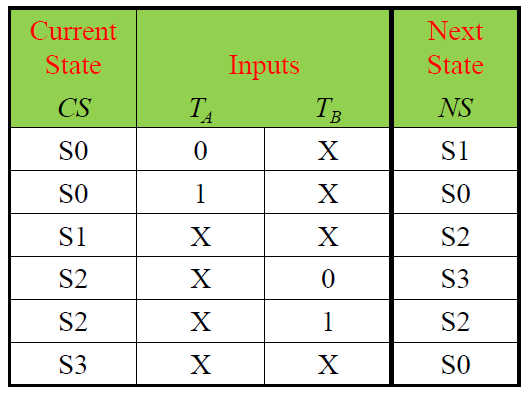
\includegraphics[scale=0.6]{状态转移表.png}
			\caption{状态转移表}
		\end{figure}\par
	
	\section{可控制时长}
		控制时长有两种方法:一种是改变时钟频率来改变时长,但这样的改变实际上是等比例地拉长了状态机在所有状态下的持续时间,并不能做到单独改变某一状态下的停留时间。
		另一种方法就是通过对控制信号$T_A$与$T_B$的控制,在设定的时间将控制信号改变来达到控制时长的效果。本题采用第二种方法进行时长的控制。
		具体的做法是:控制信号在不同的时钟周期进行变化,这样就可以实现最小时长为周期,时长为n倍周期的时长可控制。具体做法请见代码。\par
	
	\section{仿真结果}
		仿真结果如图4。
		\begin{figure}[htbp]
			\centering
			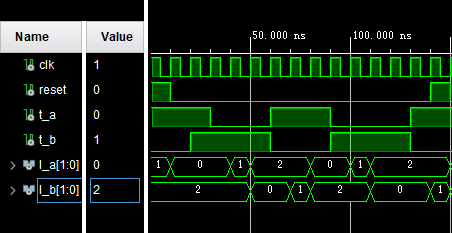
\includegraphics[scale=1.1]{仿真结果.png}
			\caption{仿真结果}
		\end{figure}\par
		图中l\_a为A方向红绿灯状态,l\_b为B方向红绿灯状态。状态编码为00-绿灯,01-黄灯,10-红灯。
\end{document}